\documentclass{article}

\usepackage{graphicx}
\usepackage{subfigure}
\usepackage[hypcap]{caption}
\usepackage{listings}
\usepackage{float}
\floatstyle{plaintop}
\restylefloat{table}
\usepackage{hyperref}

\title{Experimental Design and Data Analysis: \\Calcium, inorganic phosphorus and alkaline phosphatase levels in elderly patients}
\author{Andrew Bedard(2566978) \& Simone van Gompel(2567525) \\ Group 19}

\begin{document}

  \maketitle

  \section{Introduction}
    In this paper the process of analysing a certain dataset is laid out.
    The dataset used is calcium.dat, which can be found at \url{http://www.amstat.org/publications/jse/jse_data_archive.htm}.
    This dataset is used for this project is because it has a good number of entries and enough features to be able to do data analysis on.
    In the rest of this paper the experiment is explained, the data is analysed, the found results are shown and all of this will be discussed at the end.
    In the appendix the used R code is shown.

  \section{The Experiment}
    The experiment that was set up had as goal to see if age and sex has an influence on certain concentrations in the body.
    The concentrations that were measured are:
    \begin{itemize}
      \item Alkaline Phosphatase International Units/Liter
      \item Calcium mmol/L 
      \item Inorganic Phosphorus mmol/L
    \end{itemize}
    There are 6 different labs from which the data is extracted.
    Next to these features, the sex, age, agegroup and patient observation number are recorded.
    In the calcium.dat the original data is stored with errors, in calciumgood.dat the data is already cleaned up.
    In this project only the calcium.dat data is used to explain how the cleaning up of the data is done.
    The research question we want to answer is: What influence does age have on the given concentrations in the body?

  \section{Data Analysis}
    \subsection{Preparation}
      The data needed to be prepared to be able to read it in R.
      This preparation exists of replacing the empty fields by an underscore, with this the data can be read in R.
      First off a pairs plot was made of the data to be able to see how the data relates to each other.
      In Fig\ref{fig:FirstPairs} the foremost problem is clear, the outliers in the data are big and unlogical.
      Furthermore has Lab more than 6 categories, these problems can be explained by human error.
      And lastly the lab 3 has strange measurements with the cammol, this might be because of confusion of the measurement unit.
      The following values were changed:
      \begin{itemize}
        \item Removed Ages over 110
        \item Removed Sex which is not in the category 1 or 2
        \item Removed Lab categories which are over 6
        \item Removed Phosmmol over 2
        \item Divided Cammol of Lab 3 by 10 (this is visually tested by using a pairs plot)
      \end{itemize}
      After removal the same plot is made, see: Fig\ref{fig:SecondPairs}.
      Here you can see the correlations between the features better than in Fig\ref{fig:FirstPairs}.
      \begin{figure}[H]
          \centering
          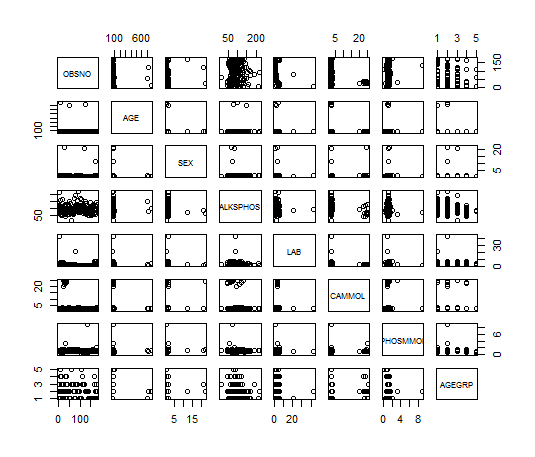
\includegraphics[scale=0.5]{../results/FirstPairs.png}
          \caption{Pairsplot of the original data}
          \label{fig:FirstPairs}
      \end{figure}
      \begin{figure}[H]
          \centering
          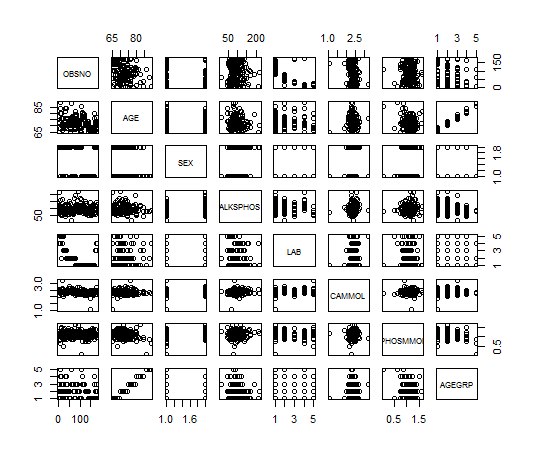
\includegraphics[scale=0.5]{../results/SecondPairs.png}
          \caption{Pairsplot of the updated data}
          \label{fig:SecondPairs}
      \end{figure}

    \subsection{Analysis}
      The feature that needs to be analyzed is age, this can be done by either using the feature age or the feature age group.
      The age group exists of 5 levels and is thus categorical.
      The different age groups are: 1=65-69, 2=70-74, 3=75-79, 4=80-84, 5=85-89 Years.
      In Fig\ref{fig:BoxAgegrp} the relation between the different concentrations and the age groups are visually represented.

      \begin{figure}[H]
          \centering
          \subfigure[Alkphos]{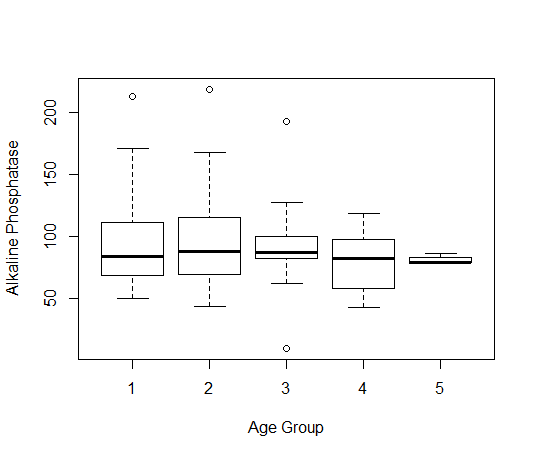
\includegraphics[scale=0.2]{../results/BoxAlksphosAgegrp.png}}
          \subfigure[Cammol]{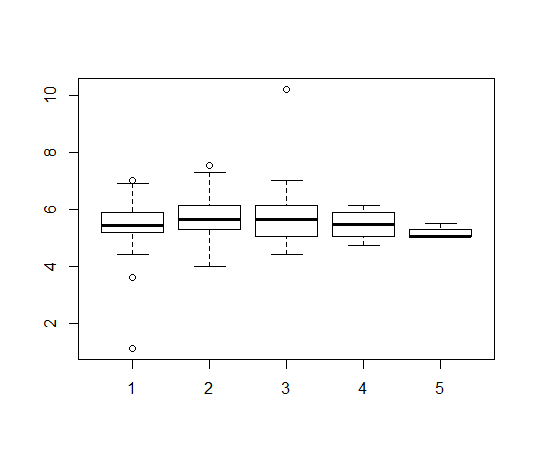
\includegraphics[scale=0.2]{../results/BoxCammolAgegrp.png}}
          \subfigure[Phosmmol]{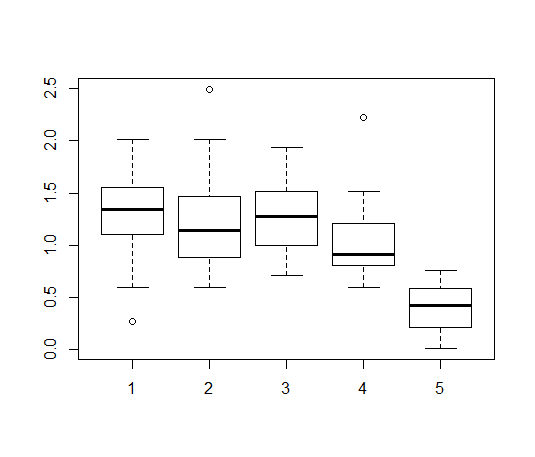
\includegraphics[scale=0.2]{../results/BoxPhosmmolAgegrp.png}}
          \caption{Boxplots of the concentrations with the age groups}
          \label{fig:BoxAgegrp}
      \end{figure}

        There is some difference between the different age groups with all of the concentrations.
        But with Alksphos the difference only seems to be in the variety of the values, the same holds for Cammol.
        For Phosmmol there does seems to be a difference in the age groups, the median drops with the older ages.
        The difference in the first two concentrations is because of the number of people in the different age groups, see Table\ref{table:Agegrp}.
        This shows that there are only three patients in the last age group and not too much in the group before that.
        This explains that the variety seems to lower with the higher age groups.
        For the rest of the analysis the last age group can be discarded, because it has not enough data to be able to analyze.
        
        \begin{table}
          \begin{center}
            \begin{tabular}{l|lllll}
            \hline
            Groups&1&2&3&4&5\\
            \hline
            Patients&56&70&38&10&3\\
            \hline
            \end{tabular}
          \end{center}
          \caption{The number of patients per age group}
          \label{table:Agegrp}
        \end{table}


  \section{Results}

  \section{Discussion}
    
  \section{R-Code}
    \begin{lstlisting}[language=R]
    \end{lstlisting}
\end{document}
